\documentclass{article}

\usepackage{polski}
\usepackage[utf8]{inputenc}
\usepackage{graphicx}
\usepackage{amsfonts}
\usepackage{amssymb}
\usepackage{amsmath}
\usepackage{listings}
\usepackage{breqn}
\usepackage{float}

\author{Maciej Pieta \and Piotr Koproń \and Jakub Woś \and Rafał Piwowar}
\date{Maj 2023}

\title{Technika Cyfrowa. \\ Ćwiczenie 3.}

\begin{document}
\maketitle
\newpage
\section{Zadanie 3a}
\paragraph{Treść zadania.}
Bazując na dowolnie wybranych przerzutnikach, zaprojektować, zbudować i przetestować synchroniczny trzybitowy licznik liczący w następujący sposób:
     0, 2, 4, 6, 1, 3, 5, 7, 0, 2 , 4 , … itd.
Inaczej mówiąc: licznik najpierw przechodzi po wartościach parzystych, a potem po wartościach nieparzystych, i znowu po parzystych, i tak w kółko.
\subsection{Ogólna idea rozwiązania}
\begin{figure}[H]
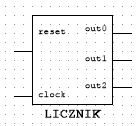
\includegraphics[width = 0.5\textwidth]{3a_blackbox}
\end{figure}
Licznik jest trzybitowy - wartość wyjściowa jest definiowana jako $1*out_{0}+2*out_{1}+4*out_{2}$.
Jako wartości wejściowe przyjmujemy zewnętrzny zegar oraz sygnał resetujący.
\subsection{Tabele prawdy}
Tabele prawdy informują o kolejnej wartości wysyłanej przez licznik, wyznaczone z wartości aktualnej.
\begin{figure}[H]
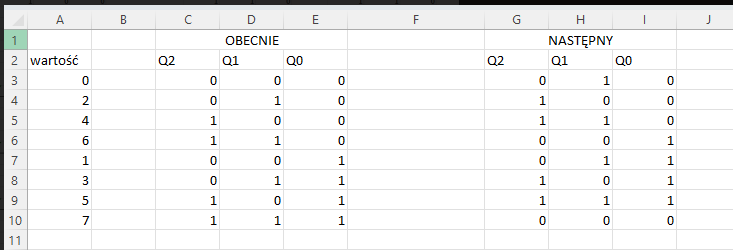
\includegraphics[width = \textwidth]{3a_tabele_prawdy}
\end{figure}
\subsection{Tabele Karnaugh}
Dokonujemy minimalizacji, w celu wyznaczenia bezpośrednich wzorów na wejścia do przerzutników, oznaczone $D_{0}, D_{1},D_{2}$.
\begin{figure}[H]
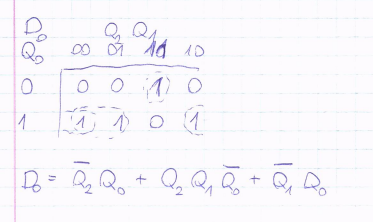
\includegraphics[width = 0.5\textwidth]{3a_karnaugh_2}
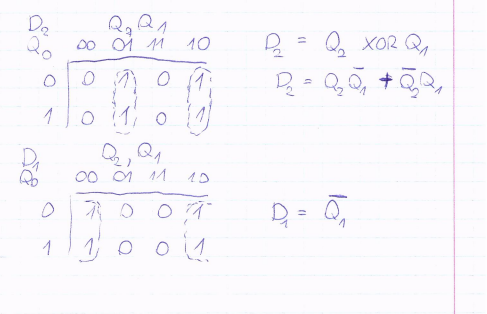
\includegraphics[width = 0.5\textwidth]{3a_karnaugh_1}
\end{figure}
\subsection{Schemat układu}
\begin{figure}[H]
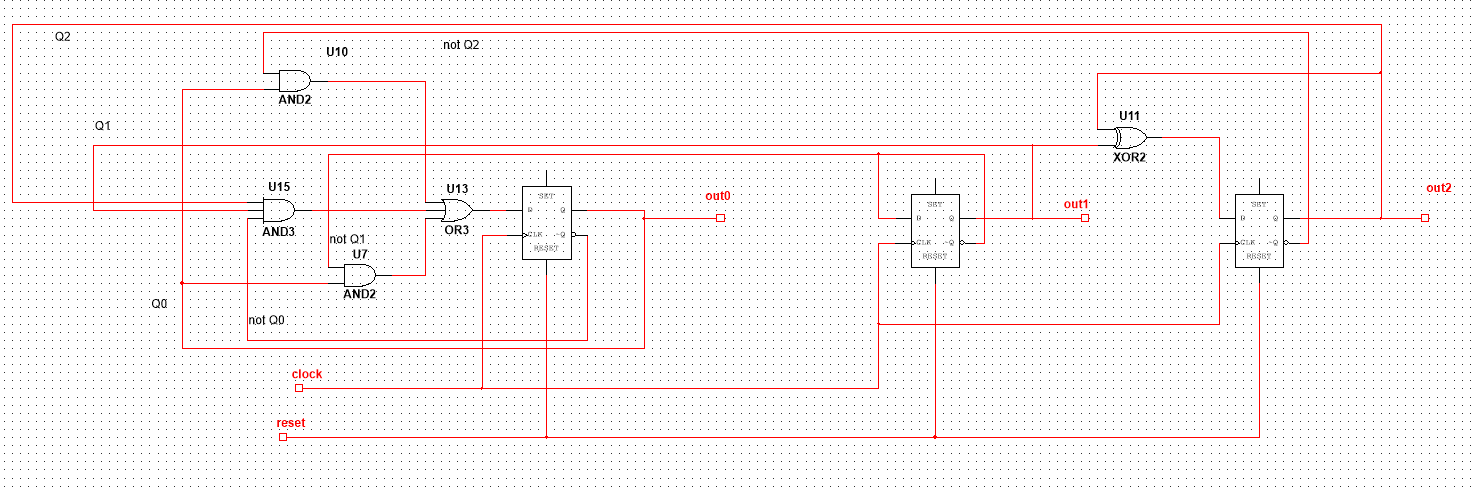
\includegraphics[width = \textwidth]{3a_uklad}
\end{figure}
Dodatkowo załączamy układ wizualizujący działanie naszego licznika.
\begin{figure}[H]
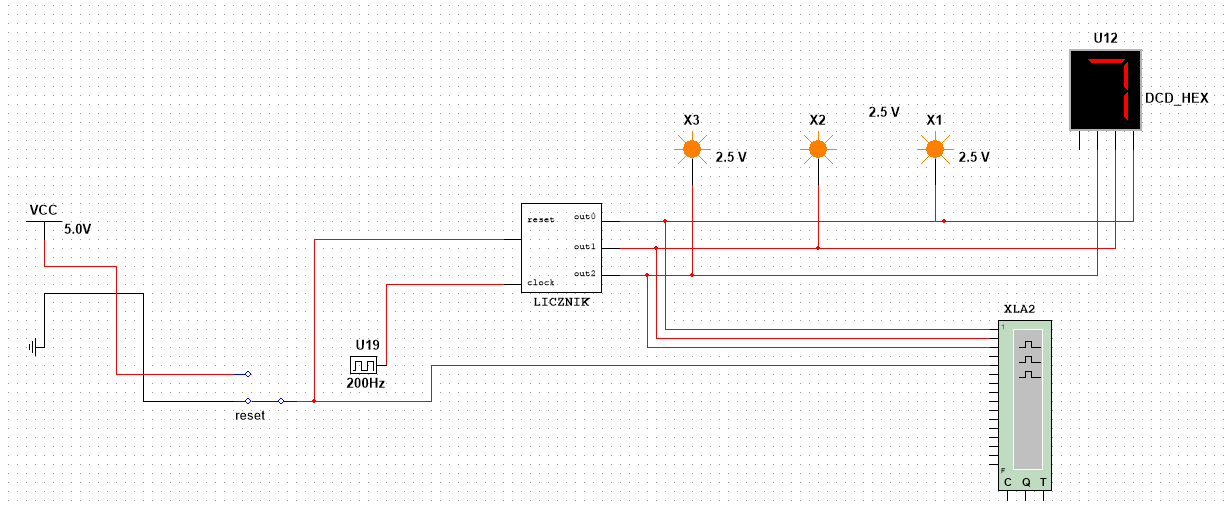
\includegraphics[width = \textwidth]{3a_wizualizacja}
\end{figure}
\subsection{Układ testujący}
Przygotowaliśmy automatyczny model testujący. Lampka błędu pozostanie zgaszona tylko jeżeli we wszystkich sytuacjach licznik zachowa się zgodnie z oczekiwaniami.
\begin{figure}[H]
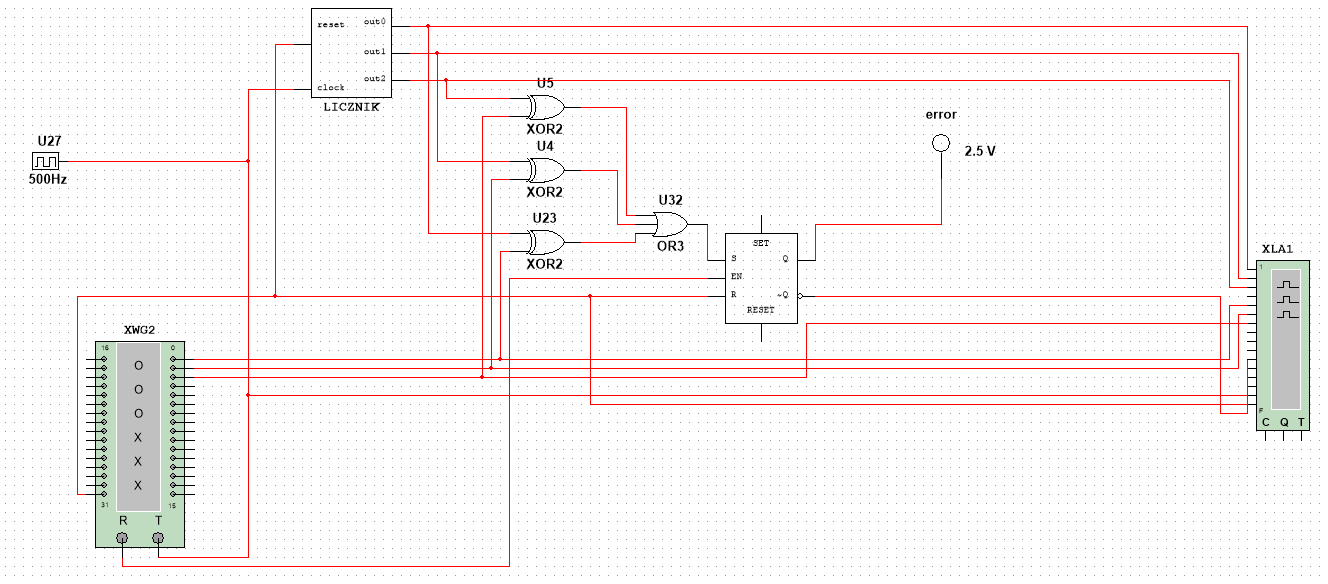
\includegraphics[width = \textwidth]{3a_tester}
\end{figure}
Ustawienia generatora słów i wyniki analizatora logicznego.
\begin{figure}[H]
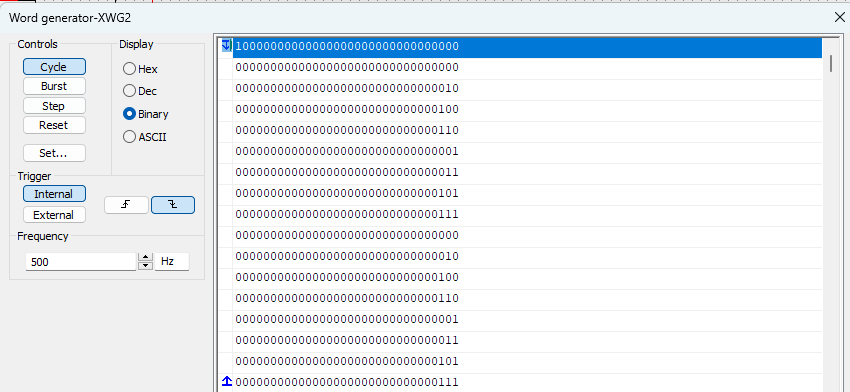
\includegraphics[width = 0.9\textwidth]{3a_generator}
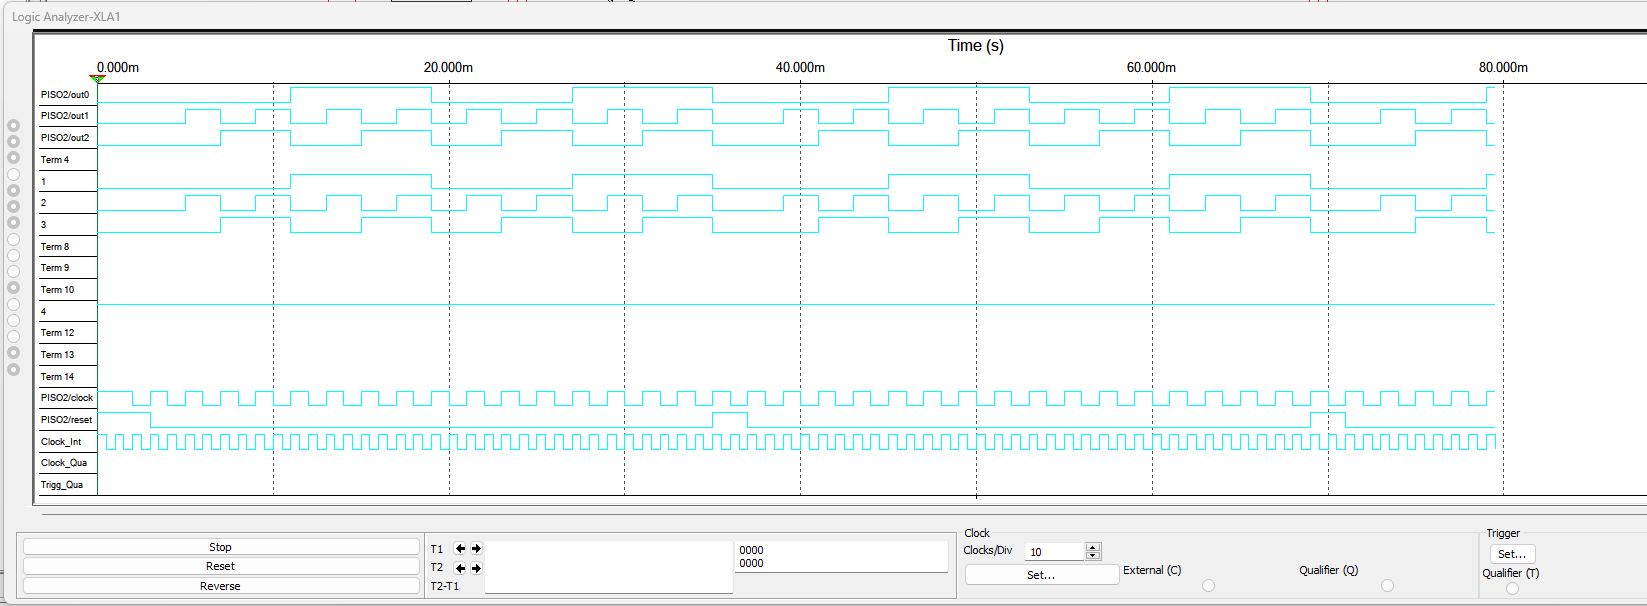
\includegraphics[width = 0.9\textwidth]{3a_analizer}
\end{figure}
Wartość oznaczona "4" stale równa 1 oznacza że lampka błędu nie świeci, czyli program działa.
\subsection{Wnioski}
\paragraph{Alternatywne rozwiązania}
Rozważaliśmy wykorzystanie przerzutnika T na zapamiętywanie najmniej znaczącego bitu, ale uznaliśmy że jednolitość przerzutników zmniejsza poziom skomplikowania układu.
\paragraph{Słowem komentarza twórczego}
Podczas przyotowywania tabeli Karnaugh, pierwotnie wyznaczyliśmy $D_{0} = \overline{Q_{2}}Q_{0} + Q_{2}Q_{1}\overline{Q_{0}} + Q_{1}\overline{Q_{0}}Q_{2}$., zanim zorienitowaliśmy się że możemy uprościć układ.
\paragraph{Zastosowania}
Licznik może być wykorzystany do synchronizacji sygnalizacji świetlnej interskrzyżowaniowo, w celu zapewnienia optymalnych warunków jazdy dla kierowców jadących zgodnie z ogarniczeniami prędkości. (Jak jedzie przepisowo, to cały czas będzie miał zielone, jak nie - to i tak będzie musiał hamować na czerwonym).
\begin{figure}[H]
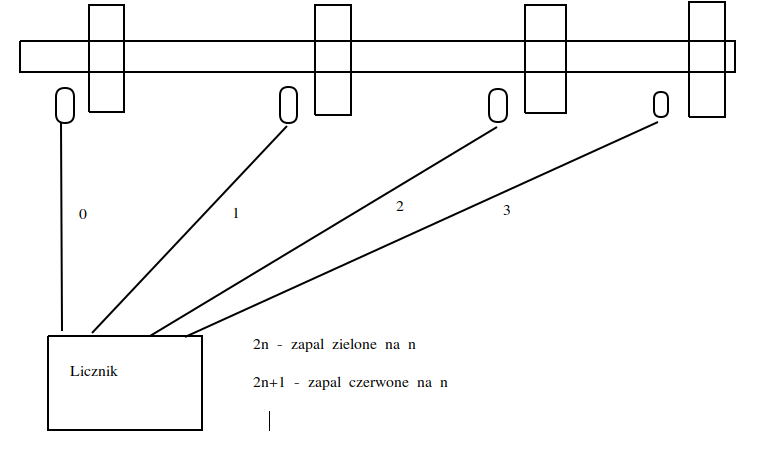
\includegraphics[width = \textwidth]{3a_swiatla}
\end{figure}
\section{Zadanie 3b}
\paragraph{Treść zadania}
Bazując na przerzutnikach "D", zaprojektować, zbudować i przetestować automat realizujący detekcję wprowadzanej na jego wejście czterobitowej wartości. Automat powinien rozpoznawać liczbę binarną: "1101". Jako źródło wprowadzanej wartości proszę użyć układu zbudowanego w ramach ćw.2b.
\newpage
\paragraph{Układ zbudowany w ramach ćwiczenia 2b}
Zgodnie z komentarzem zwrotnym do ćwiczenia 2b, zbudowany przez nas układ PISO wymagał pewnych poprawek. Załączamy tutaj poprawioną wersję.
\begin{figure}[H]
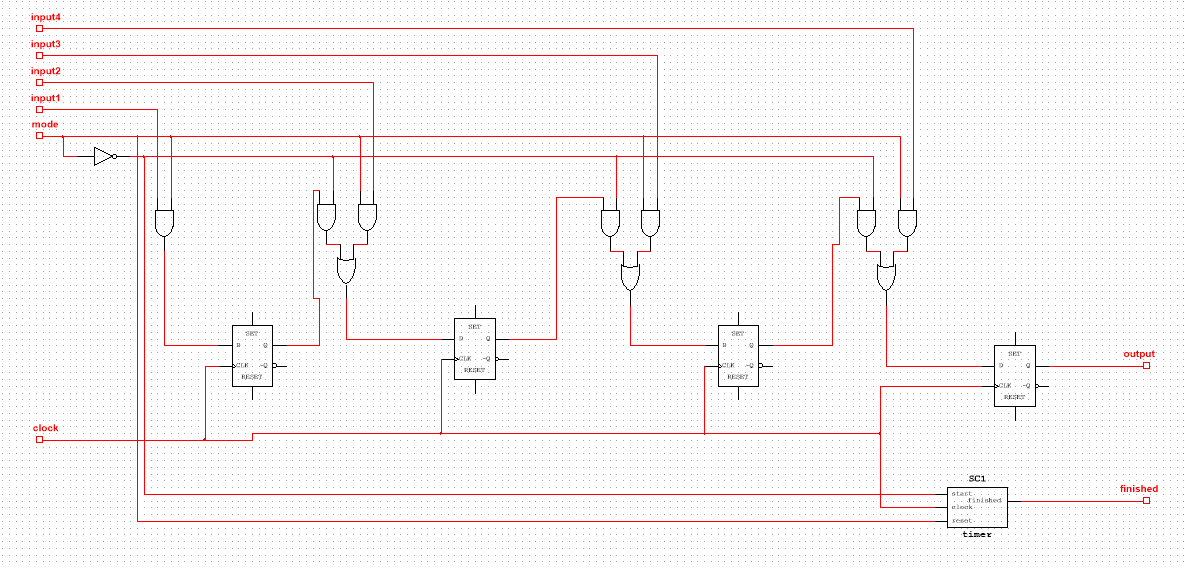
\includegraphics[width = \textwidth]{3b_2b_klaryfikacja}
\end{figure}
Układ SC1 zaimplemtowany poniżej:
\begin{figure}[H]
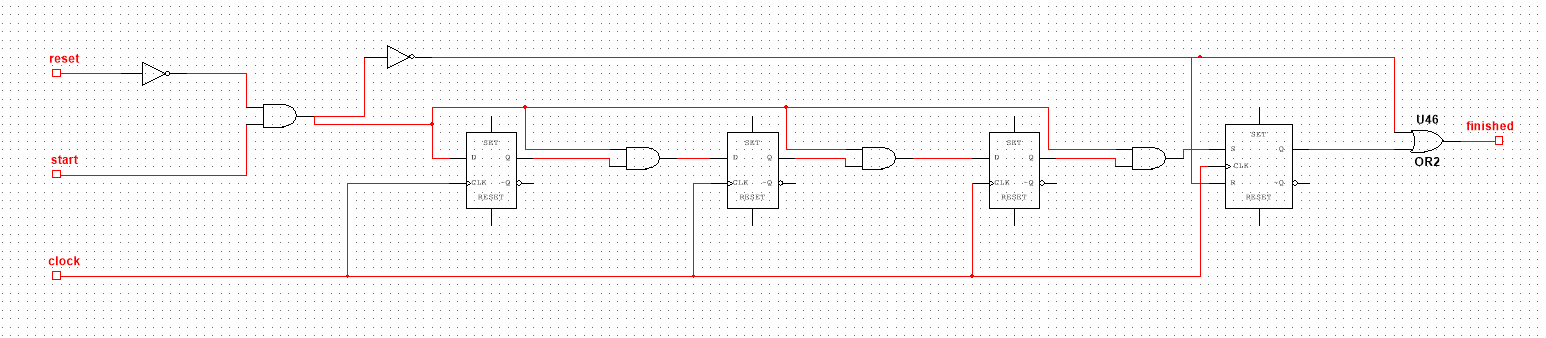
\includegraphics[width = \textwidth]{3b_SC1}
\end{figure}
\subsection{Ogólna idea rozwiązania}
Automat na wejściu przyjmuje zewenętrzy zegar, oraz sygnał wejściowy.
Oprócz tego, wprowadzony jest sygnał resetujący automat.
Na wyjściu, sygnał outY przekazuje inforamacje o tym, czy liczba "1011" została rozpoznana.
Dodatkowo, sygnały out1 i out2 pozwalają (wraz z outY) na poznanie dokładnego stanu automatu.
\begin{figure}[H]
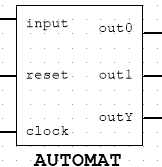
\includegraphics[width = 0.3\textwidth]{3b_blackbox}
\end{figure}
Implementujemy następujący automat:
\begin{figure}[H]
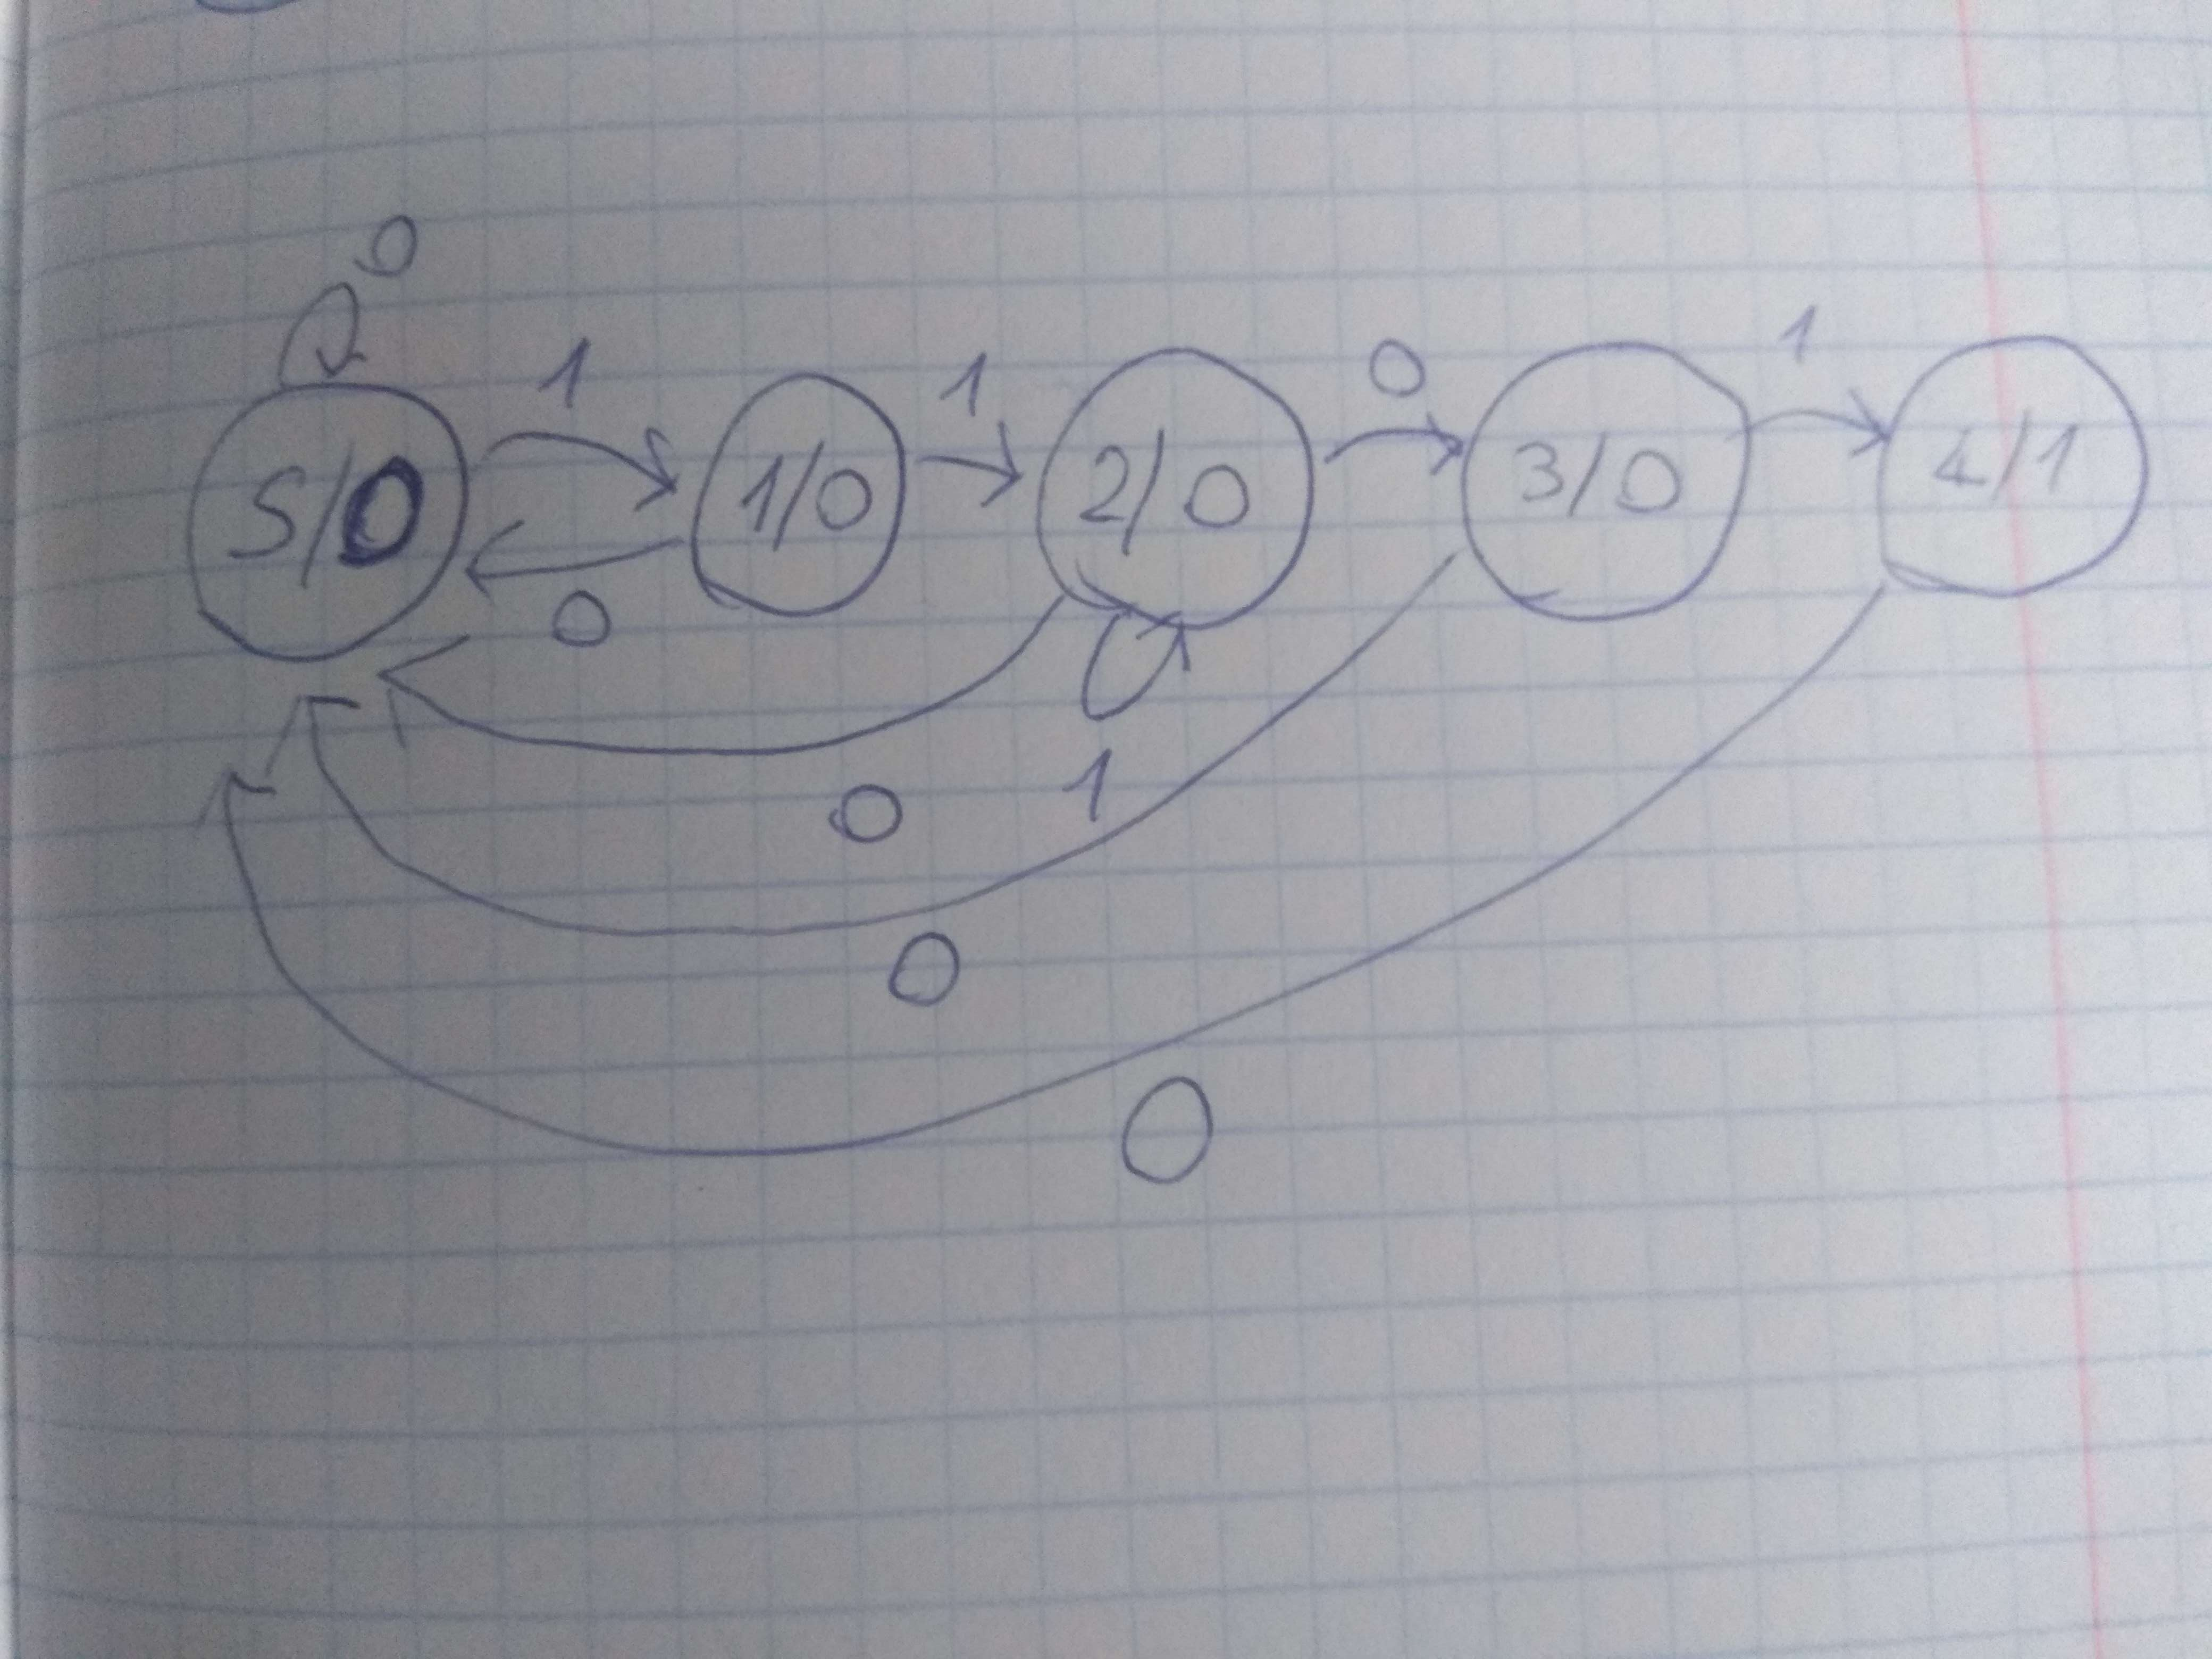
\includegraphics[width = 0.5\textwidth]{3b_automat}
\end{figure}
\subsection{Funkcje przejścia stanu}
\begin{figure}[H]
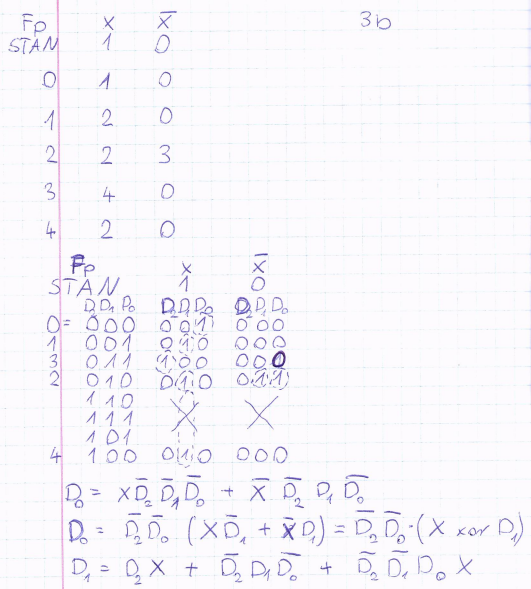
\includegraphics[width = 0.5\textwidth]{3b_przejscia}
\end{figure}
\subsection{Funkcja wyjścia}
\begin{figure}[H]
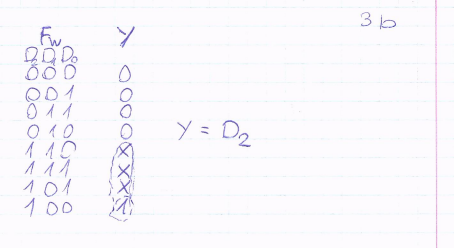
\includegraphics[width = 0.5\textwidth]{3b_wyjscia}
\end{figure}
\subsection{Schemat układu}
\begin{figure}[H]
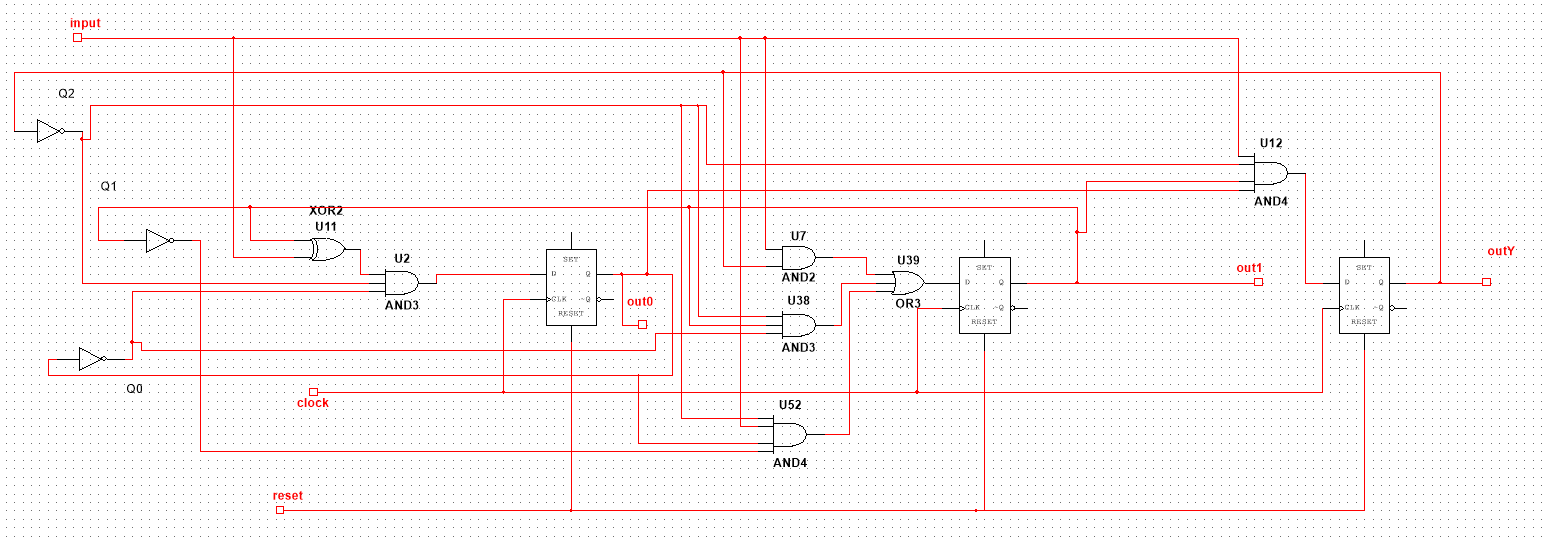
\includegraphics[width = \textwidth]{3b_uklad}
\end{figure}
W połączeniu z układem PISO z zad. 2b:
\begin{figure}[H]
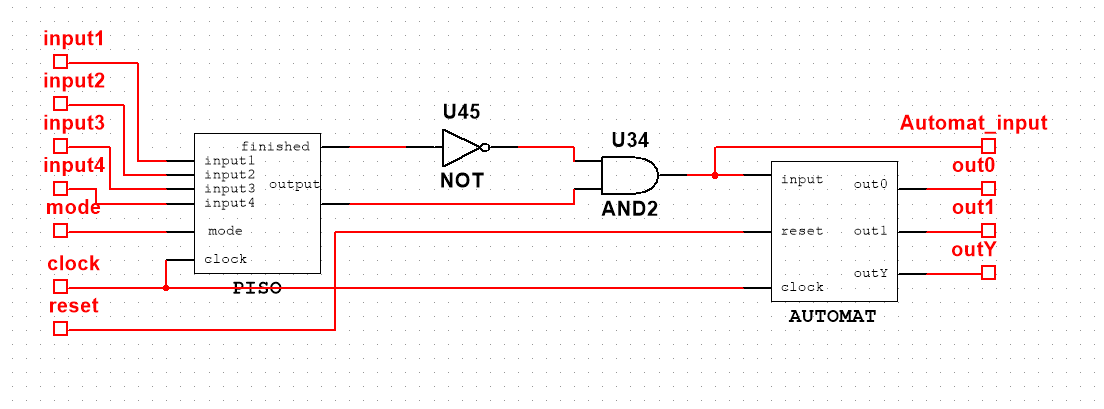
\includegraphics[width = \textwidth]{3b_uklad_z_2b_blackbox}
\end{figure}
\subsection{Układ testujący}
Przygotowaliśmy automatyczny model testujący. Lampka błędu pozostanie zgaszona tylko jeżeli we wszystkich sytuacjach licznik zachowa się zgodnie z oczekiwaniami.
\begin{figure}[H]
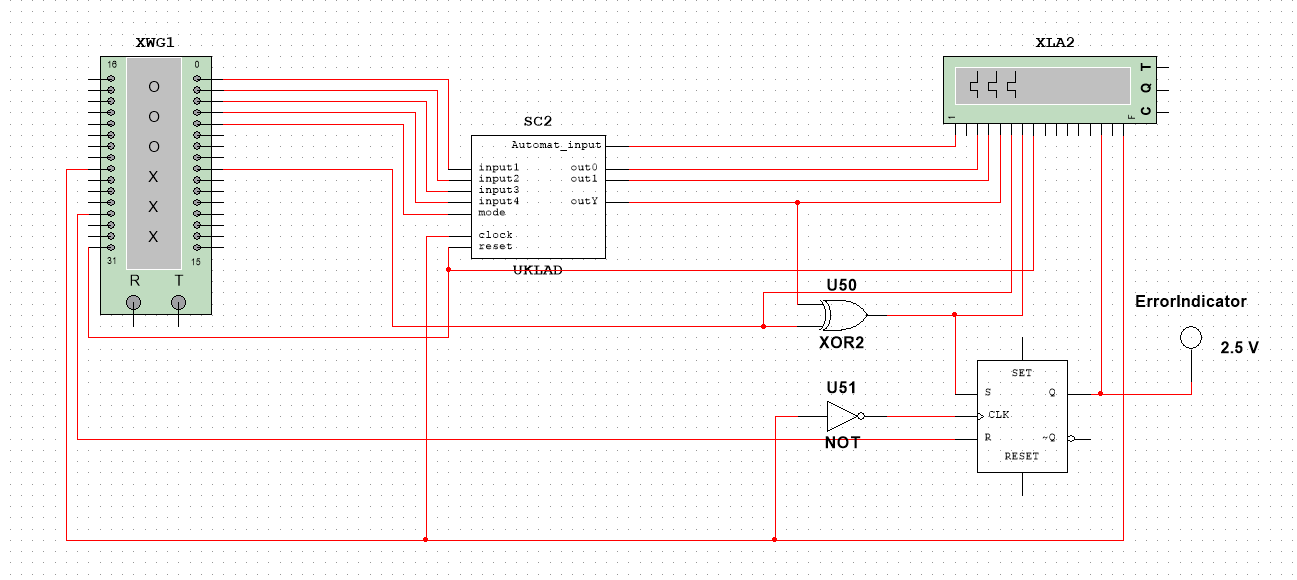
\includegraphics[width = \textwidth]{3b_tester}
\end{figure}
Załączamy kod wykorzystany do utworzenia konfiguracji generatora słów.
\begin{figure}[H]
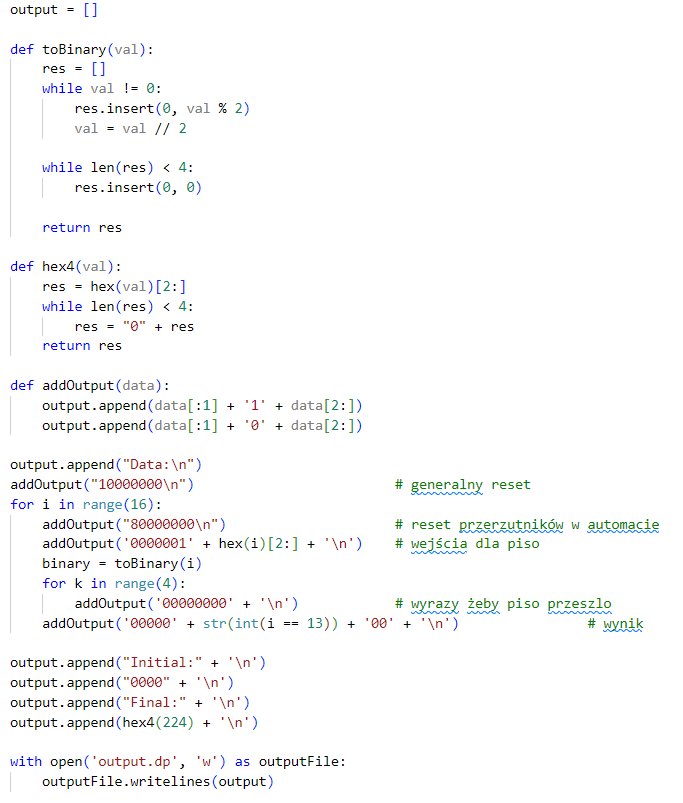
\includegraphics[width = \textwidth]{3b_code}
\end{figure}
Rezultaty z analizatora logicznego. Linia "20" stale na 0 oznacza brak błędu.
\begin{figure}[H]
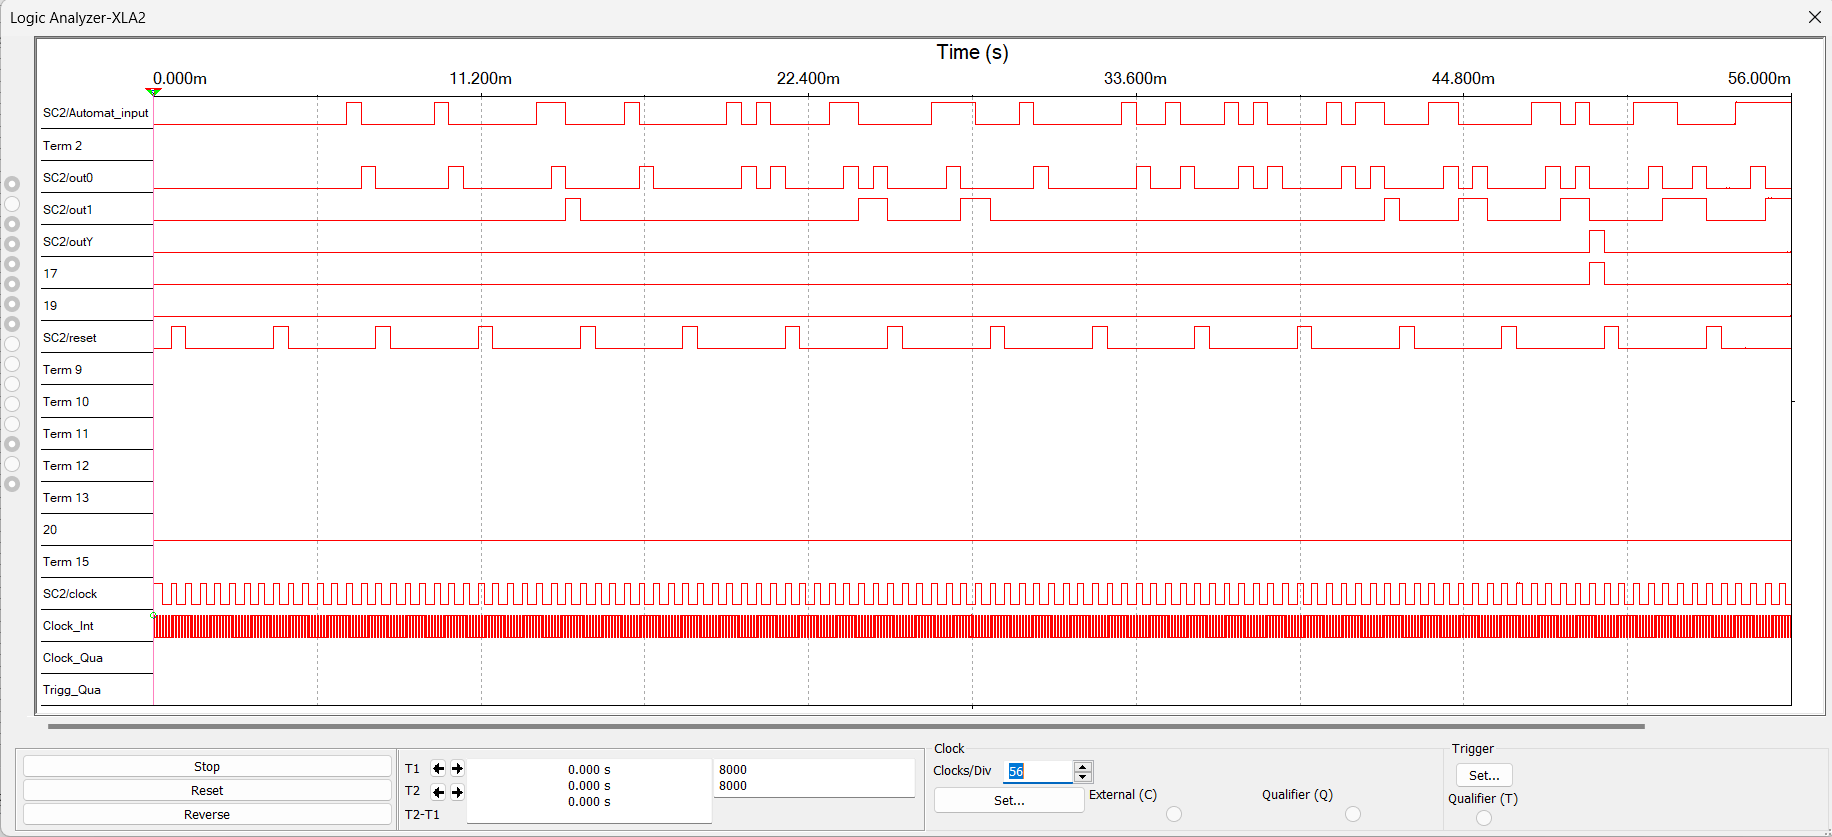
\includegraphics[width = \textwidth]{3b_analyzer}
\end{figure}
\subsection{Wnioski}
\paragraph{Alternatywne rozwiązania}
Automat realizuje detekcję "1101" z dowolnym prefiksem - alternatywny automat mógły przechodzić do stanu pułapki po otrzymaniu nieprawidłowego ciągu aż do momentu zresetowania. 
\paragraph{Zastosowania}
Automat taki może być zastosowany w drzwiach automatycznych połączonych z sensorem ruchu.
Automat najpierw sprawdza brak ruchu przez dłuższy czas ("11'), następnie ruchu, '0' - gdy ktoś podchodzi do drzwi, a następnie brak ruchu '1' - gdy ktoś zatrzymuje się przed drzwiami.
\paragraph{Zamki}
Rozważaliśmy też alternatywne zastosowanie w zamku cyfrowym - rozpoznającym kod "1101" - ale zorientowaliśmy się że osobny układ PISO z wejściem 'mode' tworzy podatność na atak, gdzie atakujący mógłby wymusić zmianę trybu aby wysłać więcej niż cztery bity.
\end{document}